\documentclass[a4paper]{article} 


%%%%%%%% DO NOT MODIFY THIS PART %%%%%%%%%%
\usepackage{url}
\usepackage[top=2cm, bottom=2cm, left=2cm, right=2cm]{geometry}
\usepackage{graphicx}
\usepackage{float}
\usepackage{minted}
\newcommand{\mytitle}[1]{\title{\textsf{\bf{#1}}}}
\date{} %
\pagestyle{empty} %
%%%%%%%%%%%%%%%%%%%%%%%%%%%%%%%%%%%%%%%%%%%%%%%%


%%%%%%%% INCLUDE MACRO HERE IF NEEDED %%%%%%%%%%
%\def\e{\varepsilon}
%%%%%%%%%%%%%%%%%%%%%%%%%%%%%%%%%%%%%%%%%%%%%%%%


%%% TITLE %%%
\mytitle{Approximating the score function using Optimal Transport}

%%%% SPEAKER (OR PRESENTATOR OF POSTER) %%%
\author{
\begin{tabular}{c}
	Quentin Giton \\ %
    Laboratoire de Mathématiques d'Orsay (LMO) \\ 
    \url{quentin.giton.pro@gmail.com}
\end{tabular}
}


\begin{document}
\maketitle
\thispagestyle{empty}


%%%% MAIN BODY -- MODIFY THIS %%%%%
We propose a novel framework to approximate the gradient flow of the free energy functional in Wasserstein space via Kantorovich potential. By reformulating the Jordan-Kinderlehrer-Otto (JKO) scheme as a sequence of convex sub-problems, our approach leverages stochastic gradient descent (SGD) to efficiently solve each minimisation problem. We study the semi-discrete case, where one measure (the source one) is seen as a discrete over the samples. In this scenario, we establish the convergence of the SGD iterates and provide error estimates. Numerical experiments illustrate the potential of our method in learning complex data distributions.


%%%% INCLUDE CO-AUTHORS NAMES HERE IF APPROPRIATE %%%%%

\paragraph{Joint work with:} Thomas Gallouët, Ziad Kobeissi.

%%%% FIGURES %%%%%

\begin{figure}[H]
	\centering
	\begin{minipage}[b]{0.45\linewidth}
		\centering
		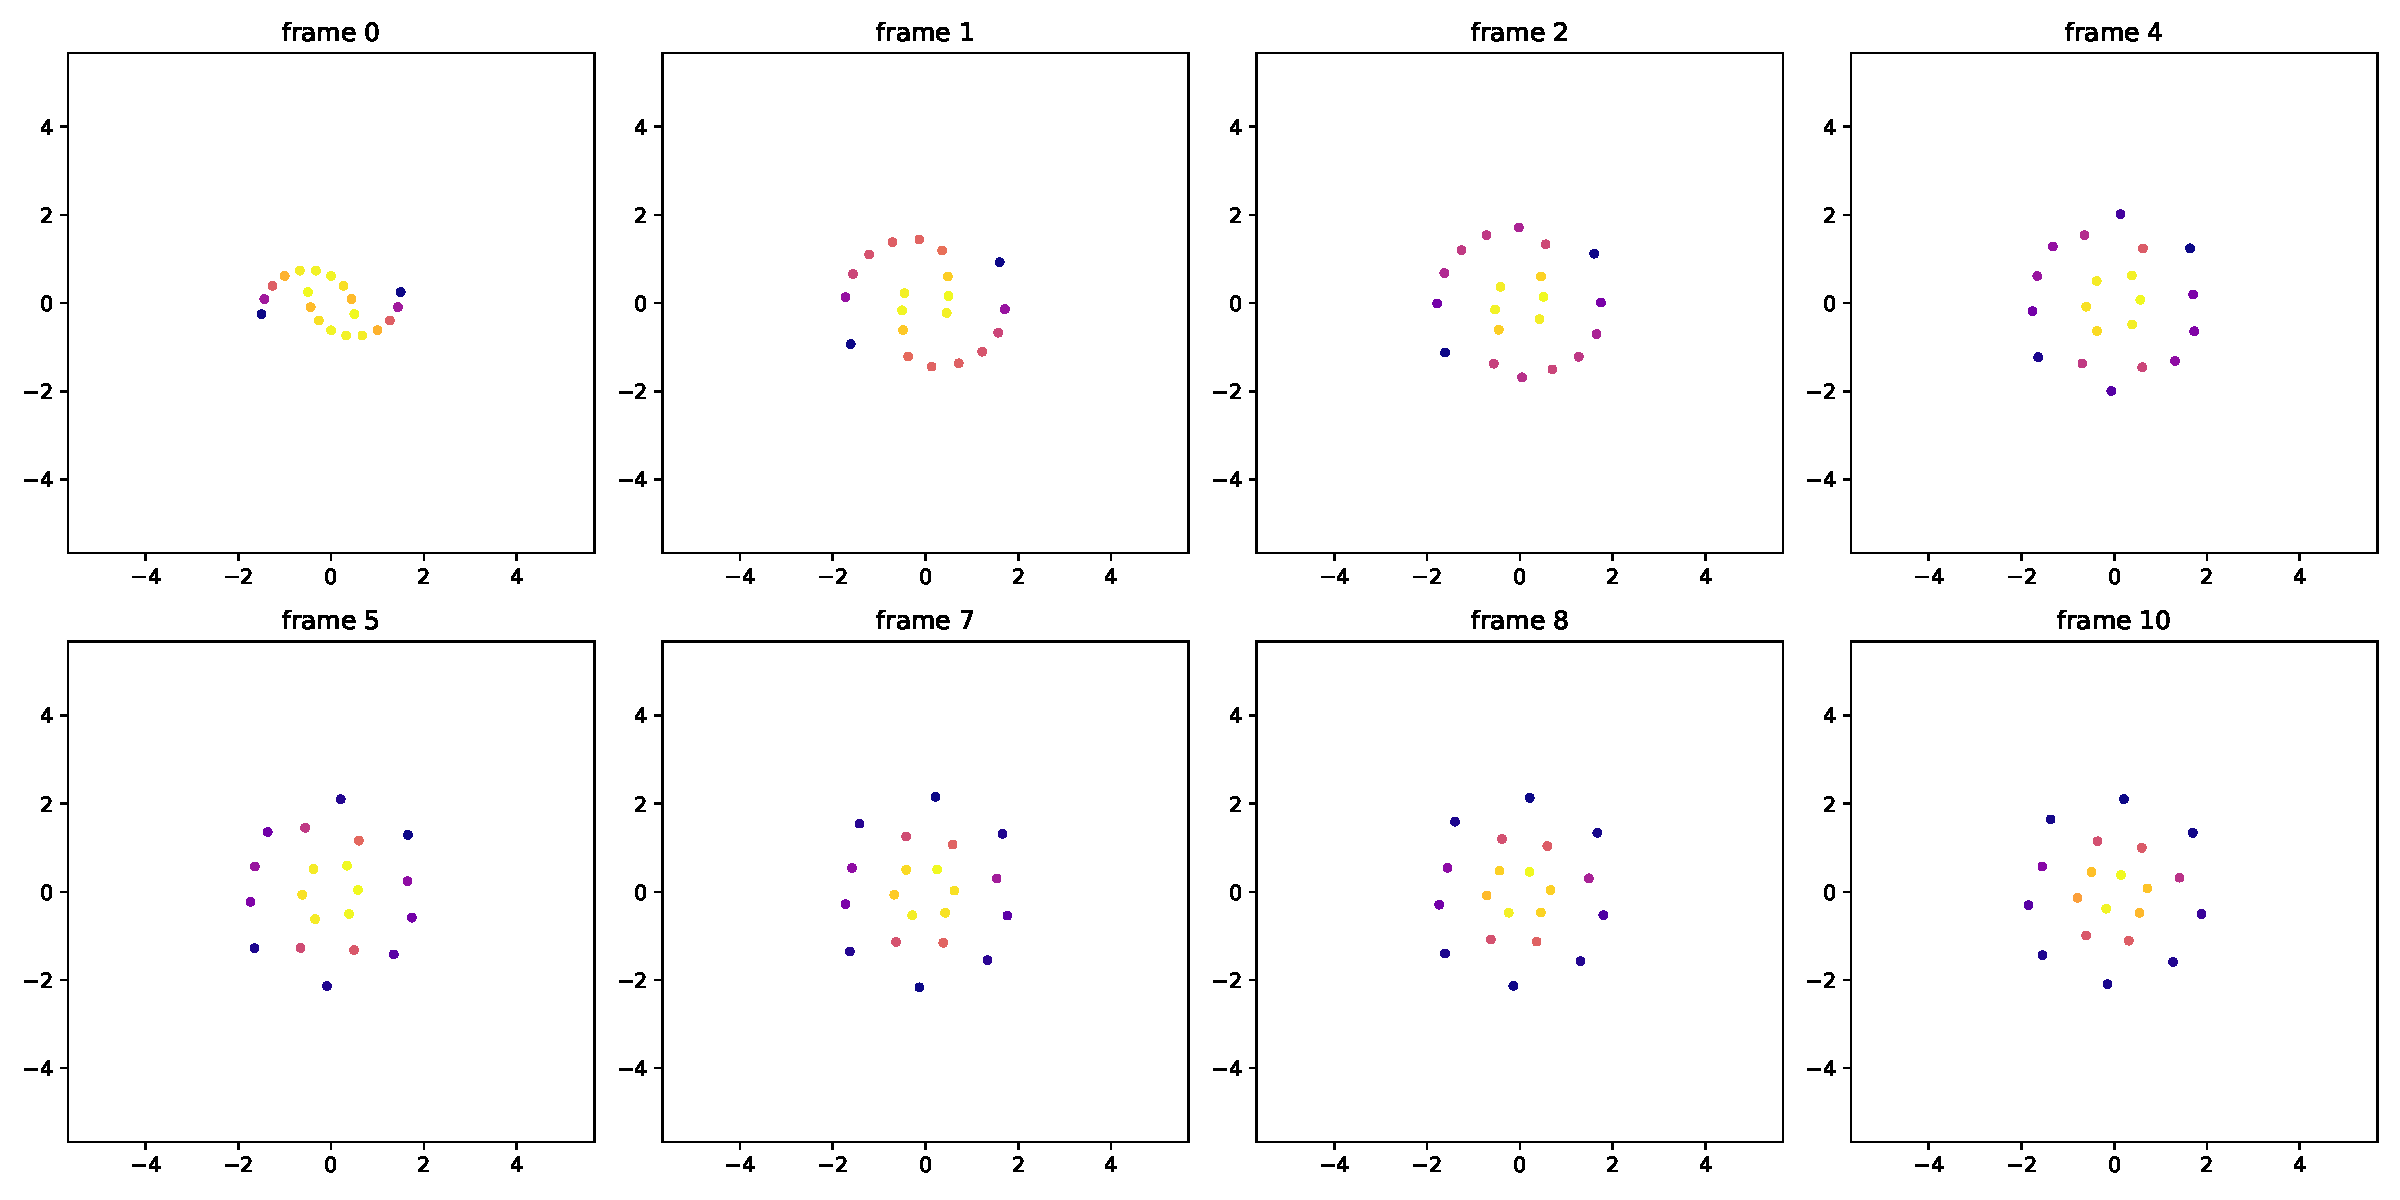
\includegraphics[width=\linewidth]{figures/forward_8frames.pdf}
		\caption{Forward: resulting points clouds after JKO steps $0$, $1$, $2$, $4$ (first row), $5$, $7$, $8$ and $10$ (second row). Simulations made with \mintinline{python}{sdot}.}
		\label{fig:forward}
	\end{minipage}
	\hspace{0.05\linewidth}
	\begin{minipage}[b]{0.45\linewidth}
		\centering
		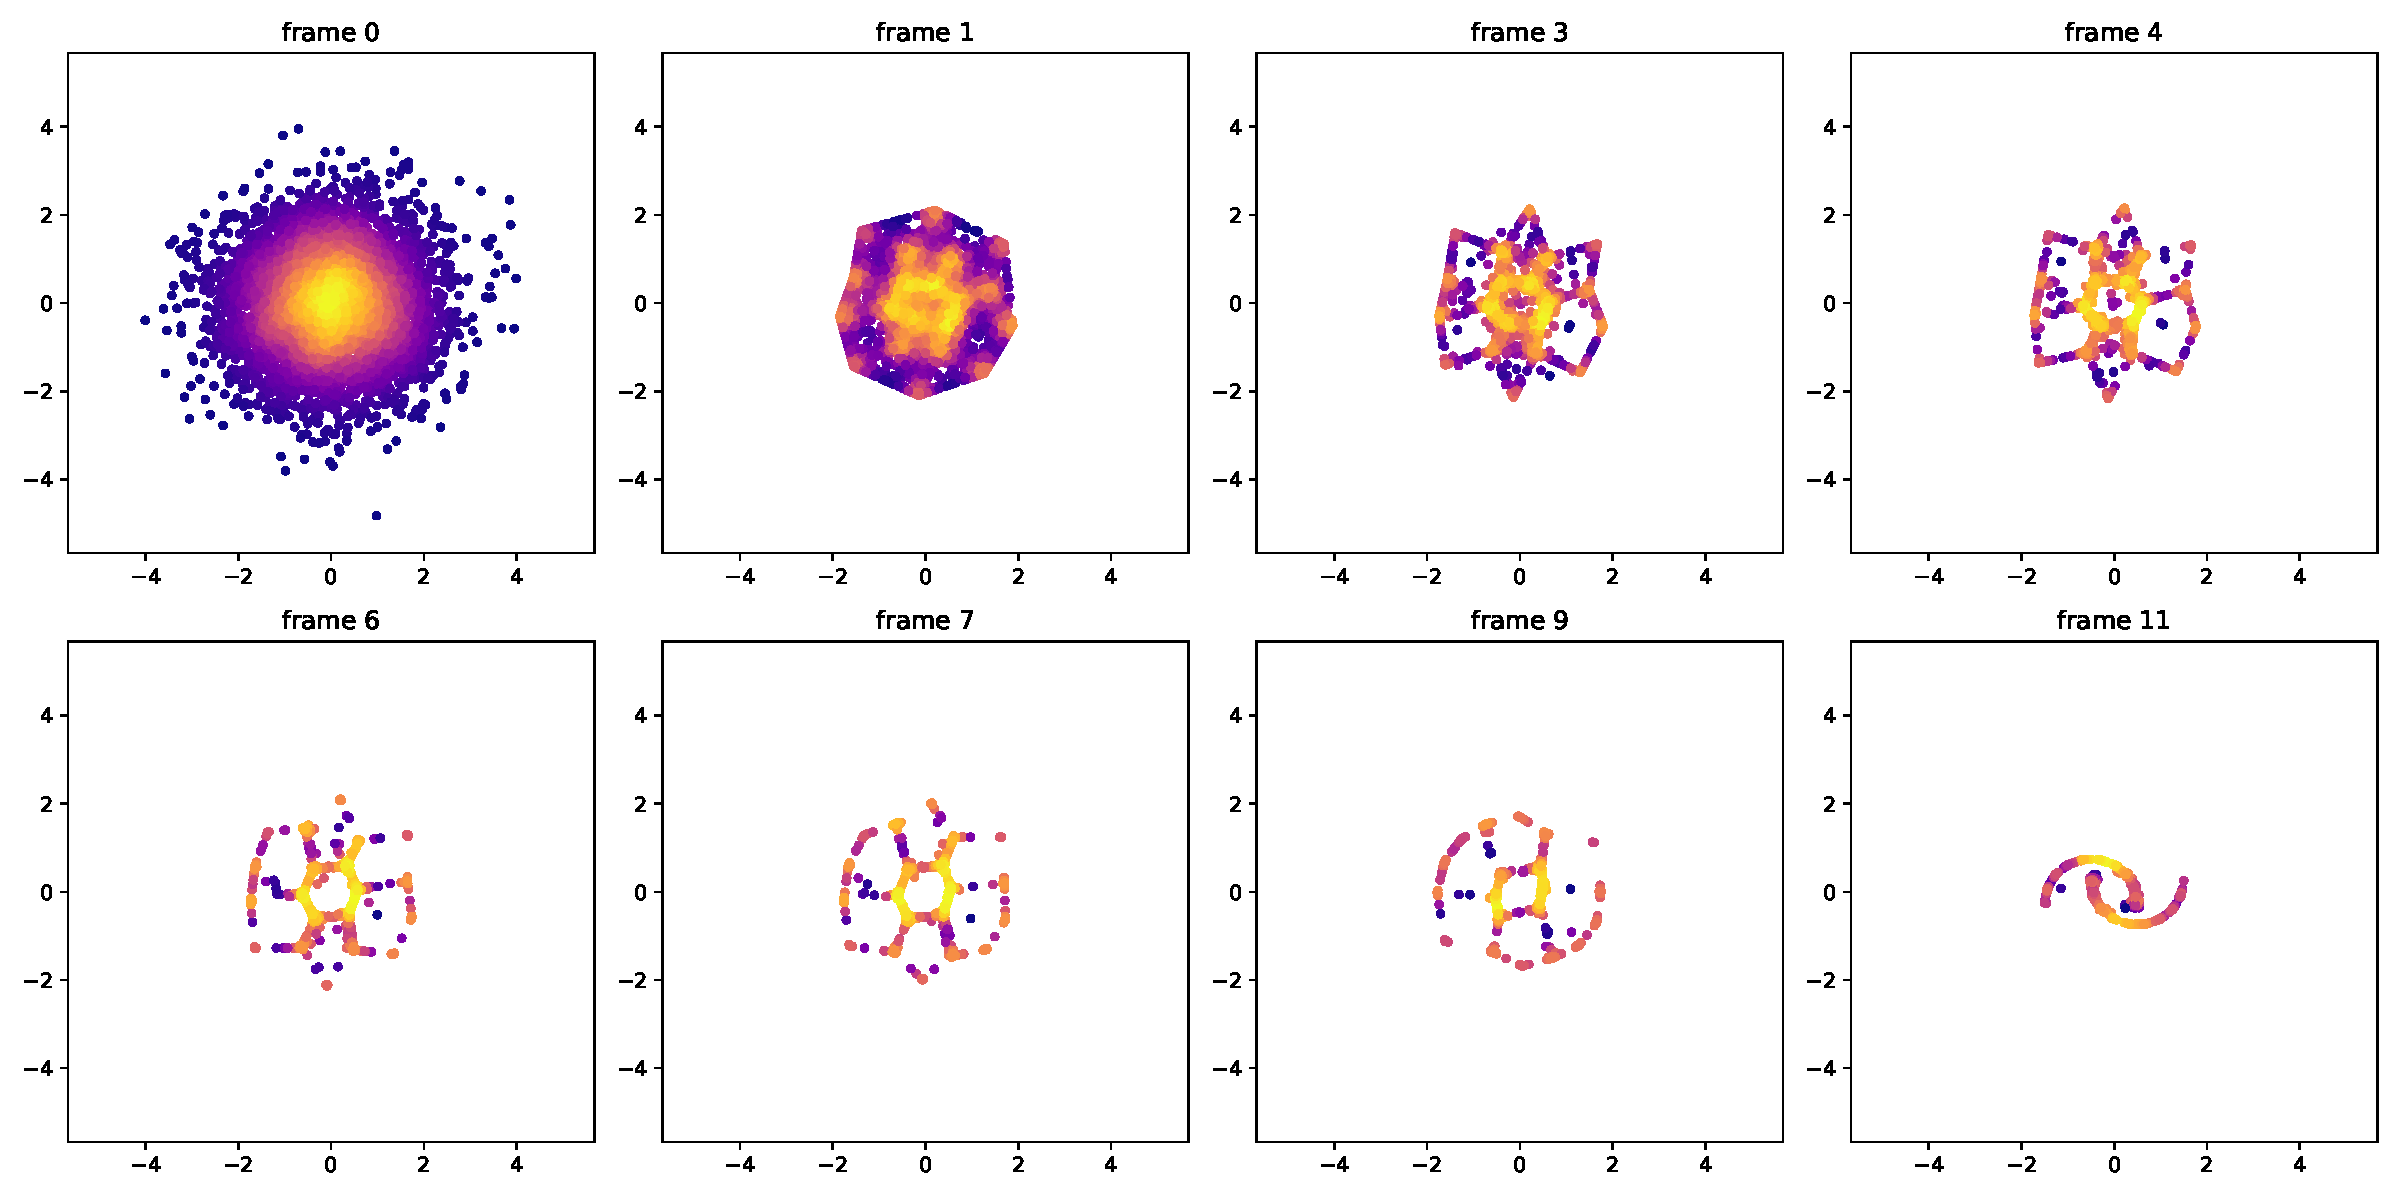
\includegraphics[width=\linewidth]{figures/convolution_backward__0_026.pdf}
		\caption{Backward: resulting points clouds after inverse steps $0$, $1$, $2$, $4$ (first row), $5$, $7$, $8$ and $11$ (second row). Simulations made with \mintinline{python}{sdot}.}
		\label{fig:backward}
	\end{minipage}
\end{figure}

%%%% BIBLIOGRAPHY -- MODIFY THIS %%%%%

\begin{thebibliography}{1}
	
	\bibitem{JKO1998}
	R.~Jordan,~D.~Kinderlehrer~and~F.~Otto.
	\newblock The Variational Formulation of the Fokker--Planck Equation.
	\newblock {\em SIAM Journal on Mathematical Analysis}, 10.1137/S0036141096303359, 1998
	
	\bibitem{fx25}
	F.~Genans,~A.~Goddichon-Baggioni,~F.-X.~Vialard~and~O.~Wintenberger.
	\newblock Stochastic Optimization in Semi-Discrete Optimal Transport: Convergence Analysis and Minimax Rate.
	\newblock {\em NeurIPS}, 10.48550/arXiv.2510.25287, 2025
	
\end{thebibliography}





\end{document}
